% ============================================================
% FENT2321 - Assignment 3
% Preliminary Blade Design and Design-Point Rotor Performance
% ============================================================

\documentclass[11pt,a4paper]{article}

% ------------------------------------------------------------
% Packages
% ------------------------------------------------------------
\usepackage[utf8]{inputenc}
\usepackage[T1]{fontenc}
\usepackage{lmodern}
\usepackage[english]{babel}
\usepackage[a4paper,margin=2.5cm]{geometry}
\usepackage{amsmath,amssymb}
\usepackage{siunitx}
\usepackage{booktabs}
\usepackage{array}
\usepackage{graphicx}
\usepackage{float}
\usepackage{caption}
\usepackage{subcaption}
\usepackage{pgfplots}
\usepackage{pgfplotstable}
\usepackage{xcolor}
\usepackage{enumitem}
\usepackage{hyperref}
\usepackage{microtype}

\pgfplotsset{compat=1.18}

\sisetup{
    per-mode=symbol,
    exponent-product=\cdot,
    output-decimal-marker={.},
    group-separator={,},
    group-minimum-digits=4
}

\hypersetup{
    colorlinks=true,
    linkcolor=black,
    citecolor=black,
    urlcolor=blue,
    pdftitle={Assignment 4 - Realistic Blade Design}
}

% ------------------------------------------------------------
% Document information
% ------------------------------------------------------------
\title{
    \textbf{FENT2321}\\[0.3cm]
    Wind Energy and Design of a Wind Turbine\\[0.5cm]
    \Large Assignment 4: Realistic Blade Design
}

\author{Markus Arntzen}
\date{}

\begin{document}

\maketitle
\thispagestyle{empty}

\clearpage
\tableofcontents
\clearpage

% ============================================================
\section{Final Blade Design and Performance}
% ============================================================

% ------------------------------------------------------------
% 1.1 Blade geometry
% ------------------------------------------------------------
\subsection{Blade geometry}

The final blade geometry obtained from the design procedure is
shown in Figure~\ref{fig:blade-geometry}. The corresponding
blade visualisation is shown in Figure~\ref{fig:blade-visualisation}.
Originally, I had bigger values for chord length, and thus, more cells saying "Too long chord lenght".
This was with $\lambda_{des} = 4.0$. After increasing $\lambda_{des}$ to the maximum constraint value of
6.0 in hopes of lowering the chord lenght to within the constrained values, this is
the best I managed. I believe misunderstanding in Assignment 3 on my part is the reason for these faulty values.
This is therefore also why the blade looks so strange and not ideal at all.

% ---------- Table: Final blade geometry ----------
\begin{figure}[H]
    \centering
    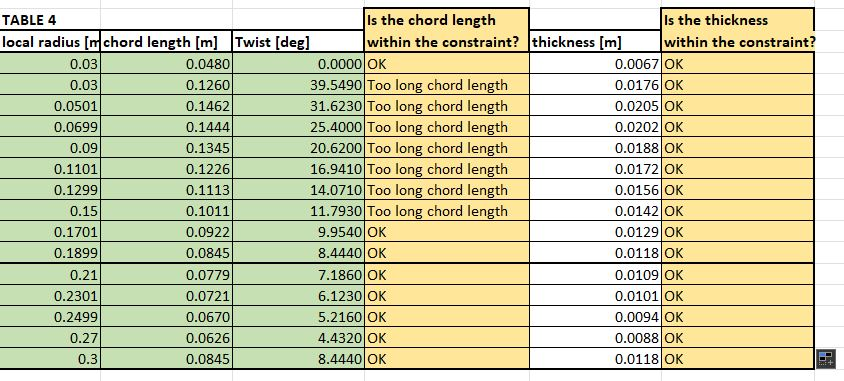
\includegraphics[
        width=0.85\textwidth
    ]{figures/geometry_table.JPG}
    
    \caption{Visualisation of the final blade geometry.}
    \label{fig:blade-geometry}
\end{figure}


% ---------- Blade visualisation ----------
\begin{figure}[H]
    \centering
    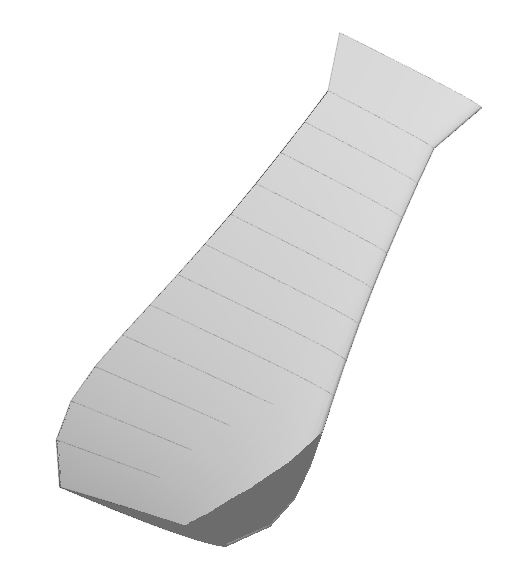
\includegraphics[
        width=0.85\textwidth
    ]{figures/blade.JPG}
    
    \caption{Visualisation of the final blade geometry.}
    \label{fig:blade-visualisation}
\end{figure}



% ------------------------------------------------------------
% 1.2 Design-point performance
% ------------------------------------------------------------
\subsection{Design-point performance}

The performance of the final blade was evaluated at the design
point using the simulation including Prandtl tip losses. The
resulting performance quantities are summarised in
Table~\ref{tab:design-point-performance}. The values for $C_P$ and $C_T$
are without the Prandtl tip losses as this achieved the biggest values in my case.
It is clearly wrong as the turbine at the design TSR will spin at 2 483 RPM, much
greater than any wind turbine and closer to the centrifuge in washing machines.
I also expected a higher torque (of course at a lower RPM) at least >1NM.

\begin{table}[H]
    \centering
    
    \begin{tabular}{l c}
        \hline
        \textbf{Quantity} & \textbf{Value} \\
        \hline
        $\lambda_{\mathrm{design}}$ & 6.5 \\
        $C_{P,\mathrm{max}}$ & ~0.345 \\
        $C_T$ & 0.842 \\
        RPM & 2 483 \\
        Torque [Nm] & 0.509 \\
        \hline
    \end{tabular}
    \caption{Performance at the design point including Prandtl tip losses.}
    \label{tab:design-point-performance}
\end{table}


% ------------------------------------------------------------
% 1.3 Performance curves
% ------------------------------------------------------------
\subsection{Performance curves}

I tried to follow the tutorial for the $C_P$ and $C_T$ simulations,
both with and without the Prandtl tip losses method. The red line in Figure~\label{fig:Cp_tipSpeedRatio}
and Figure~\label{fig:Ct_tipSpeedRatio} correspond to the Prandtl method and the blue, thinner line
is the "normal" method without Prandtl. I assume the Prandtl method graph should normally give
higher values for $C_P$ and $C_T$, and I am aware this is not the case for me.

% ---------- CP curve ----------
\begin{figure}[H]
    \centering
    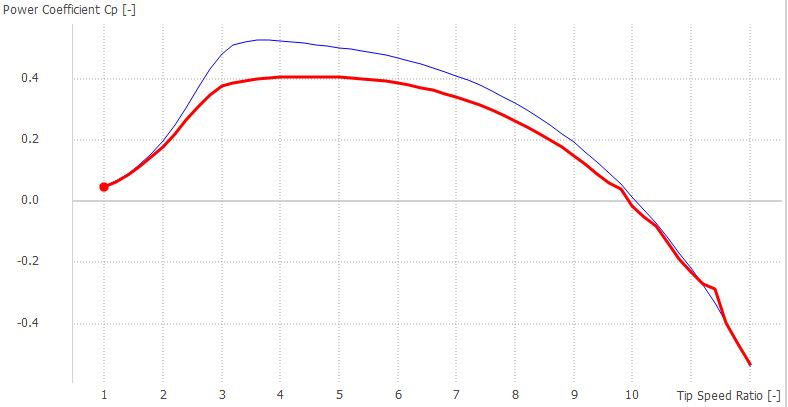
\includegraphics[
        width=0.85\textwidth
    ]{figures/Cp.JPG}
    
    \caption{Power coefficient $C_P$ as a function of
    tip-speed ratio $\lambda$, with and without Prandtl tip losses.}
    \label{fig:Cp_tipSpeedRatio}
\end{figure}


% ---------- CT curve ----------
\begin{figure}[H]
    \centering
    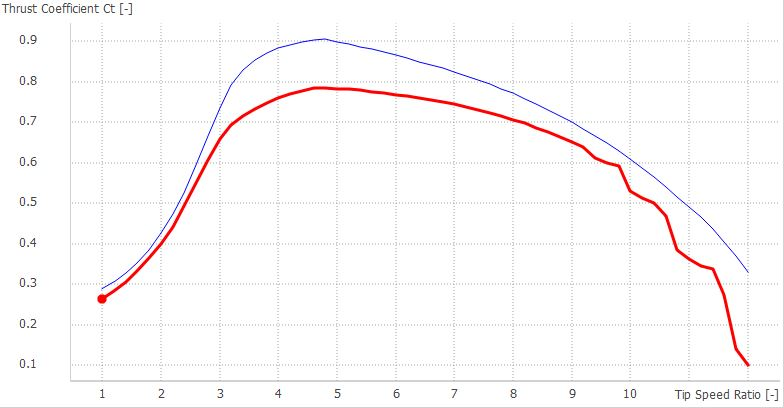
\includegraphics[
        width=0.85\textwidth
    ]{figures/Ct.JPG}
    
    \caption{Thrust coefficient $C_T$ as a function of
    tip-speed ratio $\lambda$, with and without Prandtl tip losses.}
    \label{fig:Ct_tipSpeedRatio}
\end{figure}


\subsubsection{Discussion}

I think the two graphs for $C_P$ and $C_T$ vs tip-speed ratio clearly shows
that my model has mistakes, but I am not sure where I make the mistakes.
therefore, I can not discuss any specifics.

\end{document}